% !TEX root = ../CINTA-cn.tex
%%%%%%%%%%%%%%%%%%%%%%%%%%%%%%%%%%%%%%%%%%%%%%%%%%%%%%%%%%%%%%%%%%%%
% Author: Libin Wang
% Chapter 16. Elliptic Curve
% This document was released as open source on 2026-06-18.
% Copyright 2023, Libin Wang. Creative Commons License
% This work is licensed under a Creative Commons Attribution-NonCommercial-NoDerivatives 4.0 International License.
%%%%%%%%%%%%%%%%%%%%%%%%%%%%%%%%%%%%%%%%%%%%%%%%%%%%%%%%%%%%%%%%%%%%

\chapter{椭圆曲线}
\label{chap:EC} 
\begin{introduction}
  \item 椭圆曲线
  \item 椭圆曲线上的加法
  \item 椭圆曲线上的点乘算法
\end{introduction}

\section{初识椭圆曲线}
\label{sec:ec-intro}

简单而言，所谓椭圆曲线就是满足以下方程的解，即序对$(x,y)$形成的集合：
\[y^2 = x^3 + ax + b\]

\noindent 其中，要求$\Delta = 4a^3 + 27b^2 \ne 0$，请大家先接受并记得这个常量。
如果$a$和$b$是实数，则$x$和$y$自然是实数。先看这样的点形成什么样的曲线，以建立第一印象。
使用 SageMath 做以下工作，令$a = -5$和$b = 4$，得到的椭圆曲线如图~\ref{fig:ec-1}所示。

\begin{lstlisting}
sage: a = -5; b = 4
sage: E1 = EllipticCurve(RR, [a, b])  #定义实数域上的椭圆曲线
sage: show(plot(E1, hue=.9))             #作图
\end{lstlisting}

\begin{figure}
\begin{center}
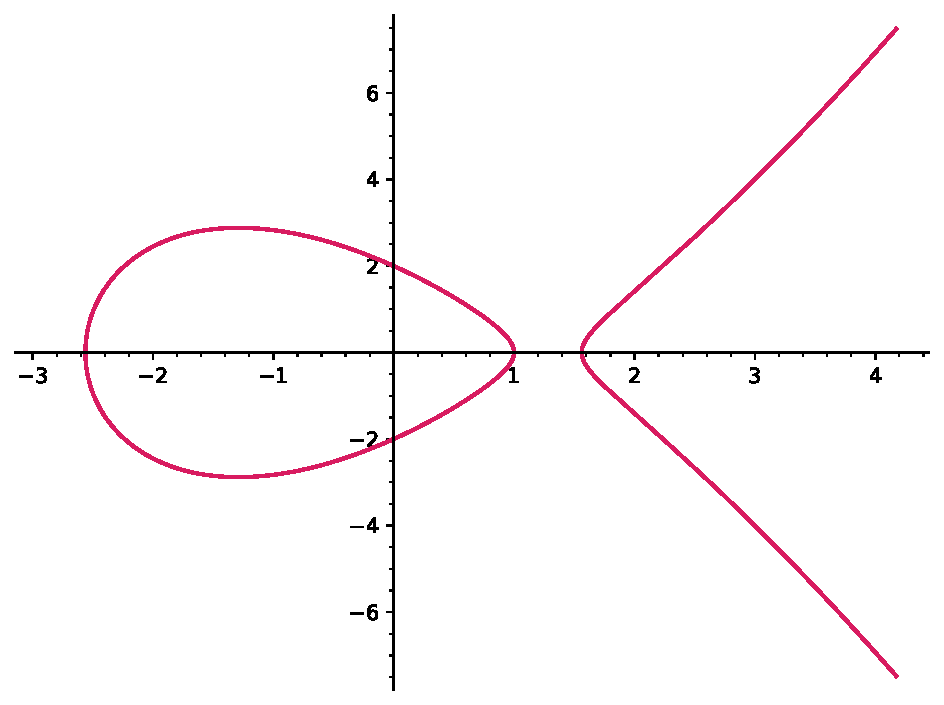
\includegraphics[scale=.5]{figures/chapt16-1-real-elliptic-curve-minus5-4.pdf}
\caption{实数域上的椭圆曲线$y^2 = x^3  -5x + 4$}
\label{fig:ec-1}       % Give a unique label
\end{center}
\end{figure}

如果改变$a$和$b$的值，可以得到其他的曲线，比如令$a = 2$和$b = 3$，得到的椭圆曲线如图~\ref{fig:ec-2}所示。
\begin{lstlisting}
sage: a = 2; b = 3
sage: E2 = EllipticCurve(RR, [a, b])
sage: show(plot(E2, hue=.9))
\end{lstlisting}

\begin{figure}
\begin{center}
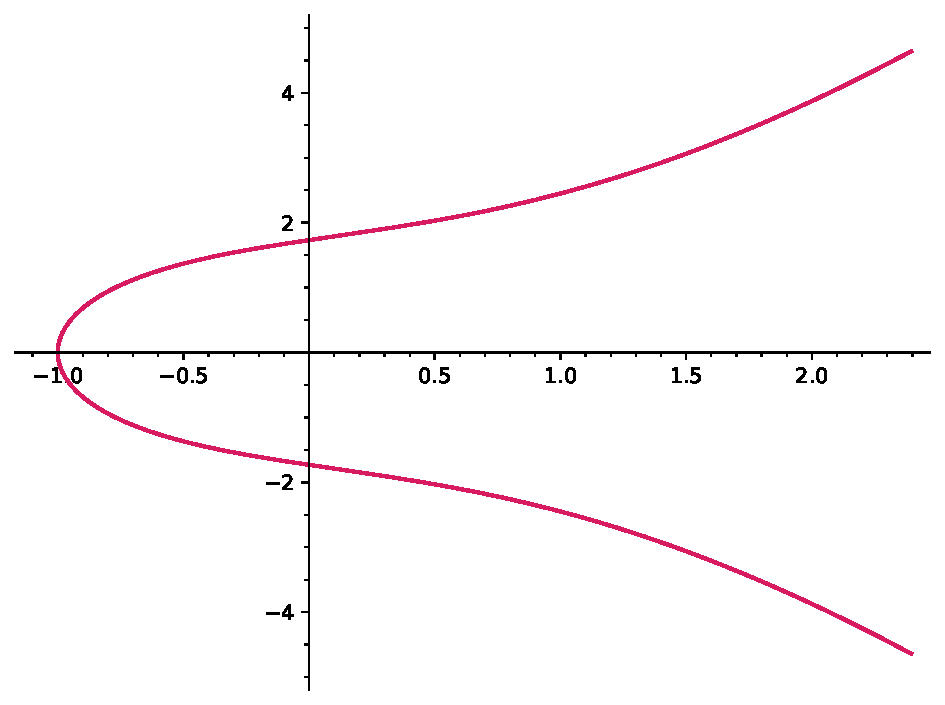
\includegraphics[scale=.5]{figures/chapt16-2-real-elliptic-curve-2-3.pdf}
\caption{实数域上的椭圆曲线$y^2 = x^3 + 2x + 3$}
\label{fig:ec-2}       % Give a unique label
\end{center}
\end{figure}

还可以选取随机的$a$和$b$，去看看曲线长什么样。比如我们完全无法预测以下曲线的模样：
\begin{lstlisting}
sage: E3 = EllipticCurve(RR,[RR.random_element(), RR.random_element()]) #RR代表实数域
sage: show(plot(E3, hue=.9))
\end{lstlisting}

通过观察以上的图，加上大家也可以利用代码构造不同的图，然后可以得到对椭圆曲线的第一印象：
长得很不椭圆！可能有一个要点大家已经注意到：\emph{曲线沿$X$轴对称}。

但是，这些落在实数域上曲线我们并不太关心，更关心的是，如果$a$和$b$落在有限域$\F$上的情形。
本节主要考虑的有限域是素域$\F_p$，$p$是素数。

比如，令$p = 137$，定义有限域$\F_p$。我们运行以下代码，得到图~\ref{fig:ec-137}。
\begin{lstlisting}
sage: p = 137 #p是一个素数
sage: F = FiniteField(p) #定义F为一种有限域，也可以用命令F = GF(p)
sage: E137 = EllipticCurve(F, [3, 8])
sage: show(plot(E137, hue=.9))
\end{lstlisting}

\begin{figure}
\begin{center}
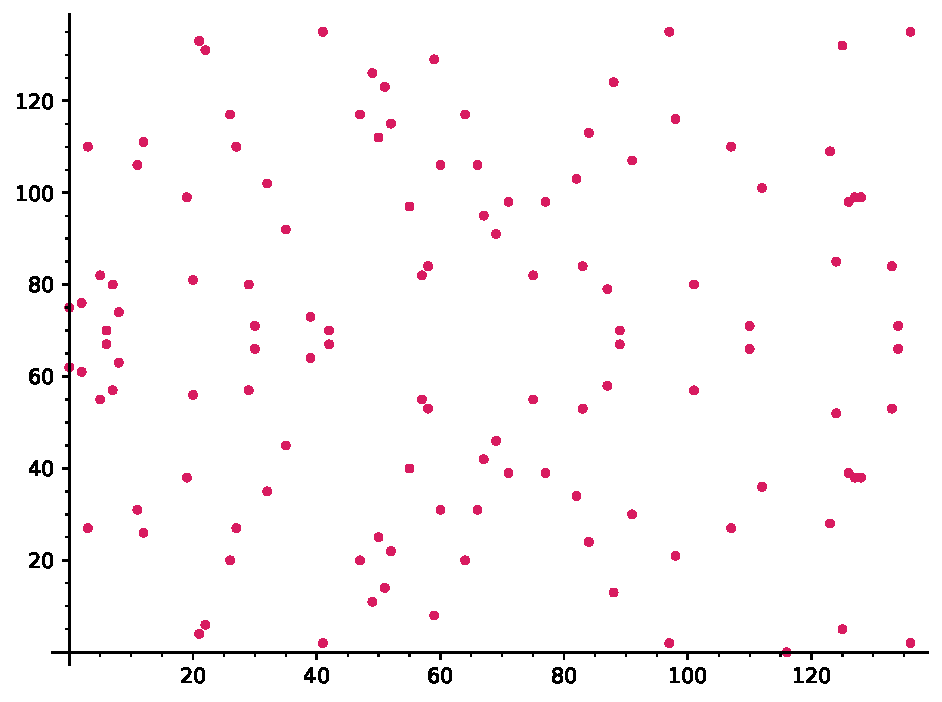
\includegraphics[scale=.5]{figures/chapt16-3-elliptic-curve-over-f137.pdf}
\caption{有限域$\F_{137}$上的椭圆曲线}
\label{fig:ec-137}       % Give a unique label
\end{center}
\end{figure}

图~\ref{fig:ec-137}所展示的椭圆曲线既不“曲”，也不成线，而是离散点的集合。
到底有多少个点呢？这是椭圆曲线研究关心的大问题。对我们而言，暂时只需要知道曲线大概的点数即可。可以使用以下命令。

\begin{lstlisting}
sage: len(E137.points())  # 所有点集合的大小
124
sage: E137.order()   #群的阶
124
\end{lstlisting}

看到这里，你至少知道椭圆曲线就是一堆“乱七八糟”点的集合，这有什么用呢？
暂时还没什么用，直到我们说，椭圆曲线上的点在加法上成群。在此先给出椭圆曲线的定义，
在此把它写成如下定理。
因为椭圆曲线上的点在对应加法上形成群，即要满足群公理，需要严谨证明，这不在本书的讨论范围之内，所以以下并不给出证明。

\begin{theorem}{椭圆曲线}{ec}
设$\F$为域，$a, b \in \F$为常数，它们使得 $\Delta = 4a^3 + 27b^2 \ne 0$。非奇异椭圆曲线 $E(\F)$
是满足方程  $y^2 = x^3 + ax + b$上的解集合 $\{(x, y) \in \F \times \F\}$ 加上一个称为\emph{无穷远点}(\emph{point at infinity})
的特殊点 $\mathcal{O}$ ，并且$E$在加法上形成一个有限交换群。
\end{theorem}

所谓无穷远点$\mathcal{O}$就是加法的单位元。这里的内涵比较丰富，稍后再进一步讨论。当前迫切的任务是要把点的加法定义出来。

\begin{remark}
以上定义还要求椭圆曲线都落在特征不为$2$和$3$的域上。因为，特征为$2$或者$3$的域会使得下一节讲解的某些计算不成立。
特征为$2$或者$3$的域上的椭圆曲线要分开独立讨论。
\end{remark}

\section{椭圆曲线群的加法}
\label{sec:ec-addition}
在定义群加法之前，先规定一些表示法。$P,Q \in E$表示曲线$E$上的两个点，注意，点是一个序对$(x,y)$。
所谓群上点的加法就是给定$P$和$Q$求$R$，使得$R = P + Q$。以下定义加法的方法从几何的角度出发，
把所有的椭圆曲线都想象为如图~\ref{fig:ec-1}或图~\ref{fig:ec-2}那样的连续的曲线。点的加法分两种情形。

第一种情形考虑两个不同的点$P$和$Q$，又称为\emph{点加}（\emph{point addition}）。
\index{点加}\index{point addition}
如图~\ref{fig:ec-add1}所示，给定两个不同的点$P$和$Q$，作$P$和$Q$的连线，
该直线与$E$相交于某个点，把这个点沿$X$轴翻转就得到了点$R$。令$R = P + Q$。

\begin{figure}
\begin{center}
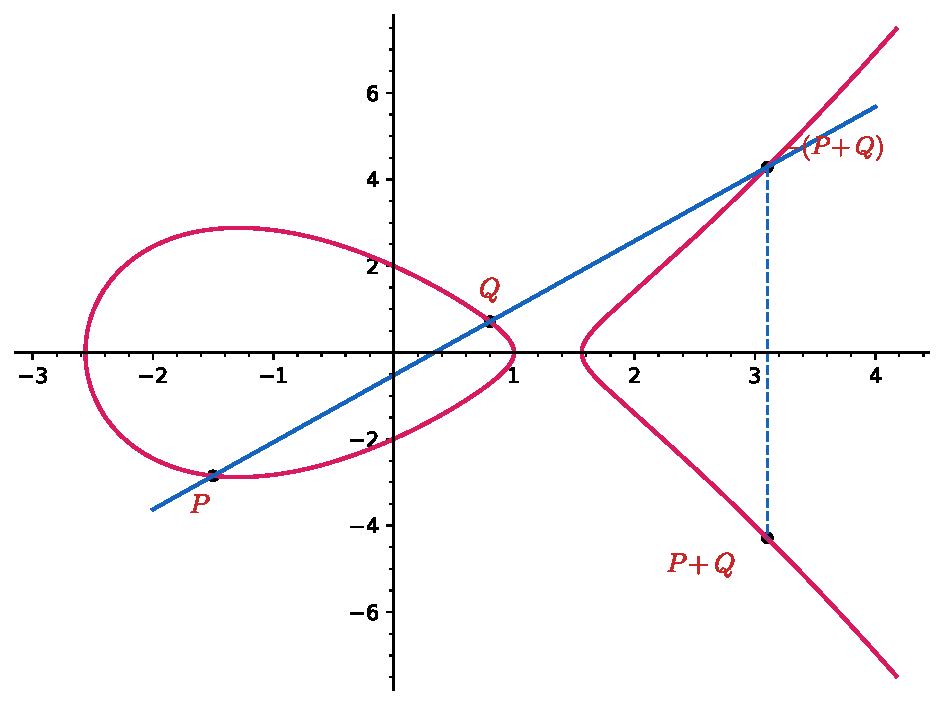
\includegraphics[scale=.4]{figures/chapt16-4-elliptic-curve-point-addition.pdf}
\caption{椭圆曲线加法-1}
\label{fig:ec-add1}       % Give a unique label
\end{center}
\end{figure}

具体到数值计算，设 $P = (x_1, y_1)$和 $Q = (x_2, y_2)$， $R = (x_3, y_3)$，则
\begin{enumerate}
\item $P$与$Q$的连线$L$的斜率$\lambda = (y_2 - y_1) / (x_2 - x_1)$ 。则直线$L$可记为： 
\[y = \lambda(x - x_1) + y_1\]

\item 求$L$ 与 $E$ 相交的另一个点。将$L$的方程代入椭圆曲线方程，即用斜率$\lambda$与$x$表达的$y$代入方程：
  	    \[(\lambda(x - x_1) + y_1)^2 = x^3 + ax + b\]
    	   \noindent 整理可得
    	\[0 = x^3 - \lambda^2 x^2 + \cdots \]

% Trey提醒这里不是三个不同的根，而且理由也不是代数基本定理。    	
 \item 因为以上方程是一个三次方程，所以它有三个根，于是有：
 \[x^3 - \lambda^2 x^2 + \cdots  =  (x - x_1)(x - x_2)(x - x_3 ) =
   	      x^3 - (x_1 + x_2 + x_3) x^2 + \cdots   =  0 \]
   	      
 \item 可得：$x_3 = \lambda^2 - x_1 - x_2$，进而可得$y_3 = \lambda(x_1 - x_3) - y_1$。注意，这里已经做了值的翻转！	  
\end{enumerate}

%注意，难道所有三次方程都一定有三个不同的根，不能是重根吗？好问题，答案是：
%三次方程的判别式 $\Delta=4a^3 + 27b^2 \ne 0$ 已经确保了重根不会出现。这个讨论请参考课后习题。
%错误理解！

第二种情形，考虑$P = Q$时的加法，又称为\emph{倍点}（\emph{point doubling}）。
\index{倍点}\index{point doubling}
如图~\ref{fig:ec-add2}所示，此时，只给定了一个点$P$，我们要计算$R = P + P$。

\begin{figure}
\begin{center}
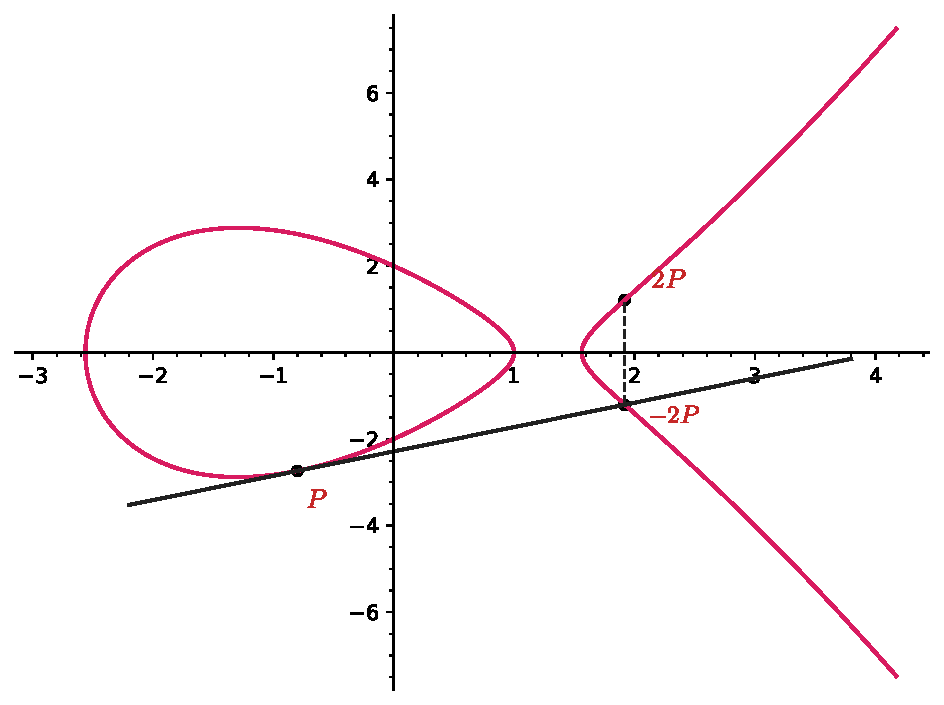
\includegraphics[scale=.5]{figures/chapt16-5-elliptic-curve-point-doubling.pdf}
\caption{椭圆曲线加法-2}
\label{fig:ec-add2}       % Give a unique label
\end{center}
\end{figure}

首先，沿点$P$作曲线的切线，与$E$相交于某点，然后沿$X$轴翻转该点就得到$R$。具体计算公式如下：
\begin{enumerate}
\item $\lambda = (3x_1^2 + a) / 2y_1$

\item $ x_3 = \lambda^2 - 2x_1$，$y_3 = \lambda(x_1 - x_3) - y_1$
\end{enumerate}
以上计算最重要是要考虑$\lambda$。$\lambda$就是经过点$P$在曲线$E$上的切线的斜率，
根据隐式微分：
\[2y \frac{dy}{dx} =  3x^2 + a\]
所以
\[\lambda = \frac{dy}{dx}  = \frac{3x_1^2 + a}{2y_1 }  \]
余下推导过程作课后练习。

\begin{thinking}
之前强调过此时域的特征不为$2$，请思考，如果此时域的特征为$2$，$\frac{3x_1^2 + a}{2y_1 }$会是什么情况？
此时需要重新提及第~\ref{chap:group}章命题~\ref{pro:grp_expo}之上那个不大会引起注意的“注”。%~\ref{rem:scaler-vs-group-element}。
\end{thinking}

讲到这里大家是否会提出这样的异议：没错，如果椭圆曲线是在实数域上$\mathbb{R}$，以上推导基本没什么问题，
但是我们知道，如果椭圆曲线落在$\mathbb{F}$上，曲线是离散点的集合，那么做连线、切线、求斜率等等，这一系列我们都做不到啊！？
说得没错，这一系列几何意义确实很难体现。但是，不要忘记，在实数域$\R$上曲线的点加法
无非就是用到了域上的加法与乘法。所有的域都可以做加法、乘法运算。所以，定义任意域上的椭圆曲线
的点加法，只需要把以上定义的所有相关操作“平移”到特定域上即可！

\begin{example}
设$a = 3$，$b=4$，定义有限域$\mathrm{GF}(137)$上的椭圆曲线方程：$y^2 = x^3 + 3x + 4$。给定两个点$P = (x_1,y_1)=(18,100)$，$Q=(x_2,y_2)=(20,114)$，求$R = P + Q$。

解法如下：
\begin{itemize}
\item 求$\lambda = (y_2 - y_1) / (x_2 - x_1) = (114 - 100)/(20 - 18) = 7$。
\item $x_3 = \lambda^2 - x_1 - x_2 = 7^2 - 18 - 20 = 11$
\item $y_3 = \lambda(x_1 - x_3) - y_1 = 7(18-11) - 100 = 86$ 
\end{itemize}
注意，所有加减乘除都是域上运算。所以，$R =(x_3,y_3)=(11, 86)$。大家可以通过 Sage 进行验证：
\end{example}

\begin{lstlisting}
sage: p = 137
sage: F = GF(p)
sage: E137 = EllipticCurve(F, [3,4])
sage: P = E137(18,100)
sage: Q = E137(20,114)
sage: R = P + Q; R
\end{lstlisting}

请注意，椭圆曲线群的定义之所以写为定理，是因为其中的群结构属性需要证明。即需要证明
椭圆曲线$E$的点在以上加法上满足：封闭性、存在单位元、存在逆元、结合律和交换律。其中，
结合律的证明并不显然，而是较为复杂的证明，本书略过。

无穷远点到底是什么？我们知道$\mathcal{O}$是群的单位元，也就是说如果$P$与$Q$互为逆元，$P + Q = \mathcal{O}$。
而$P$与$Q$互为逆元意味着，它们曲线上是沿$X$轴对称的两个点，那么它们的连线永远是垂直于$X$轴的线。
与$X$轴垂直的线与曲线在哪里还能相交出一个点呢？理论上就只能在无穷远的地方。
直观上，$\mathcal{O}$就代表所有垂直于$X$轴的线在曲线上的交点。图~\ref{fig:ec-InfPot}展示了这种直观。

在 SageMath 中，无穷远点可以这样表达：
\begin{lstlisting}
sage: p = 137
sage: F = GF(p)
sage: E137 = EllipticCurve(F, [3,4])
sage: ZeroPoint = E137(0)
\end{lstlisting}

\begin{figure}
\begin{center}
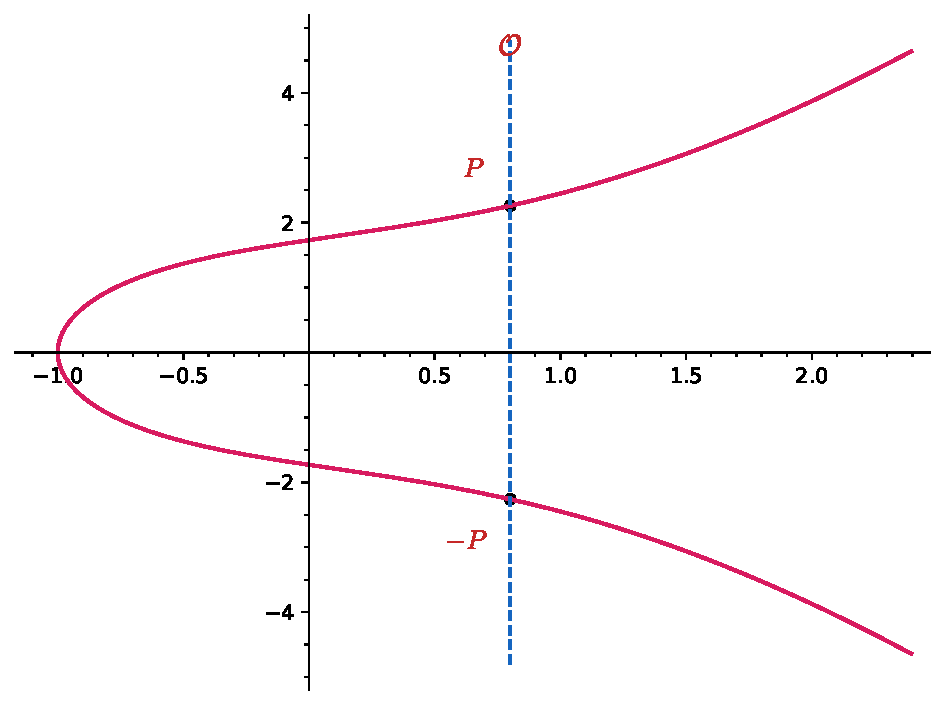
\includegraphics[scale=.4]{figures/chapt16-6-elliptic-curve-inverse-and-infinity.pdf}
\caption{椭圆曲线群的逆元与无穷远点}
\label{fig:ec-InfPot}       % Give a unique label
\end{center}
\end{figure}

要求三次方程的判别式 $\Delta=4a^3 + 27b^2 \ne 0$ 是为了确保方程$x^3 + ax + b = 0$不会出现重根，此时椭圆曲线
就不会出现\emph{奇异点}（\emph{singular points}）。\index{奇异点}\index{singular points}
要理解所谓奇异点，可先直观地认识当$\Delta = 0$时曲线
的形状。比如，通过 SageMath 可以画以下曲线：

\begin{lstlisting}
sage: x, y = var('x, y') #定义两变量
sage: implicit_plot(x^3 - y^2 == 0, (x,-3,3), (y,-3,3))  # 画曲线y^2 = x^3
sage: implicit_plot(x^3 -3*x + 2 - y^2 == 0, (x,-3,3), (y,-3,3)) # 画曲线y^2 = x^3 - 3x + 2
\end{lstlisting}
%%%%
%%f(x,y) = x^3 -12*x + 16 - y^2 another curve with singular points
%%%
图~\ref{fig:ec-singular1}显示的曲线有一个不平滑的折点，而图~\ref{fig:ec-singular2}的曲线则自己与自己相交，产生一个交点，这些
点就是所谓的奇异点。存在奇异点的曲线
都不符合我们对椭圆曲线的要求。

\begin{figure}
\begin{center}
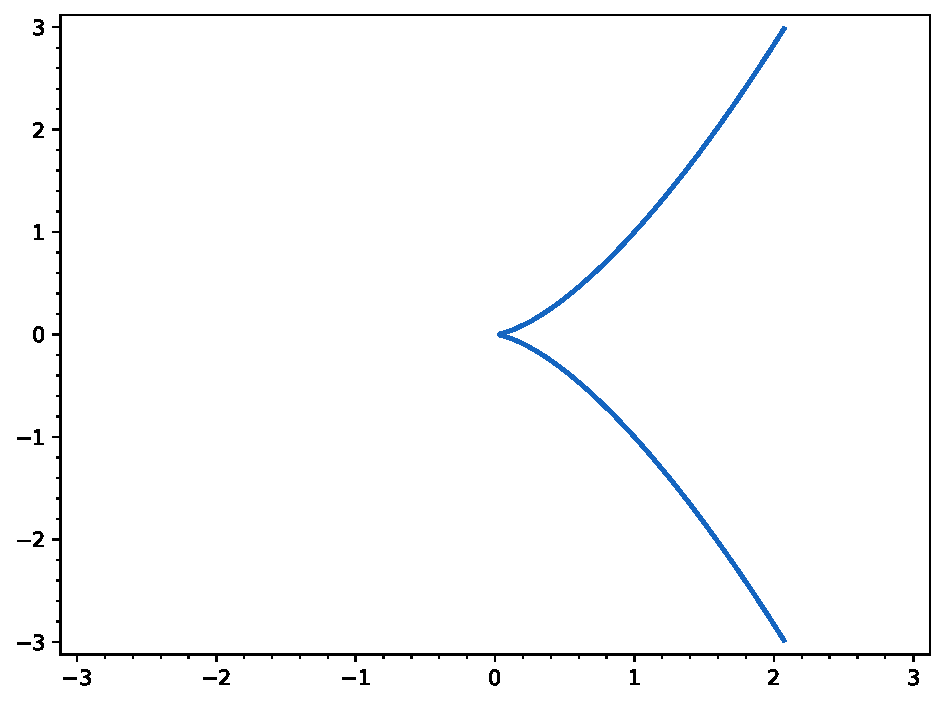
\includegraphics[scale=.5]{figures/chapt16-7-singular-cubic-cusp.pdf}
\caption{带奇异点的曲线-1}
\label{fig:ec-singular1}       % Give a unique label
\end{center}
\end{figure}

\begin{figure}
\begin{center}
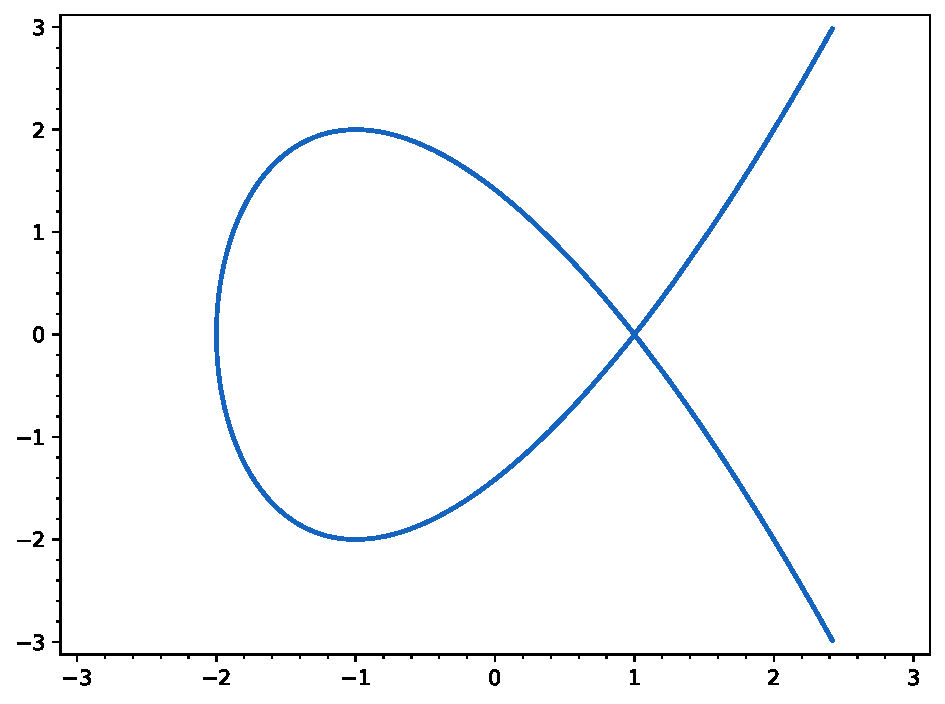
\includegraphics[scale=.5]{figures/chapt16-8-singular-cubic-node.pdf}
\caption{带奇异点的曲线-2}
\label{fig:ec-singular2}       % Give a unique label
\end{center}
\end{figure}

给定椭圆曲线$E(\F)$上的一个点$P$，根据以上计算法则，理论上可以计算出$E(\F)$上所有的点。
问题是，在最开始如何找到$E(\F)$上的一个点？

\begin{theorem}{Hasse定理}{hasse}
设$p$为素数，$E(\F_p)$是有限域$\F_p$上的椭圆曲线，
则$p + 1- 2 \sqrt{p}  \leq \vert E(\F_p) \vert \leq p + 1+ 2 \sqrt{p} $。
\end{theorem}
Hasse定理没有告诉我们椭圆曲线$E(\F_p)$上点的准确个数，但是它暗示说椭圆曲线$E(\F_p)$上的点很多，大致有$(p + 1) - \epsilon$那么多，其中
$\vert \epsilon \vert \le  2\sqrt{p}$。因此，随机挑选一个序对$(x,y)$都以很大的概率是
椭圆曲线上的点。要相信概率！做法如下：均匀随机选取$x \in \F_p$，根据椭圆曲线方程计算出$y^2$
（注意这里只是表示一个值），然后
判断$y^2$是否模$p$的二次剩余，如果是，则求平方根得到$y$。上述过程使用的算法都出现在第~\ref{chap:qr}章，
具体实现留作课后练习。

SageMath 可以方便地帮我们计算所定义椭圆曲线群的阶。
\begin{lstlisting}
sage: p = 137
sage: F = GF(p)
sage: E137 = EllipticCurve(F, [3,4])
sage: E137.cardinality()    # 等同于E137.order()
\end{lstlisting}

\section{椭圆曲线的点乘算法与离散对数问题}
对任意的$k\in \N$，给定$P$为椭圆曲线$E(\F)$上的一个点，计算
\[kP = \underbrace{P + P + \cdots + P}_k\]
\noindent 即求$k$个$P$相加得到的点，这种计算称为\emph{点乘}（\emph{point multiplication}）
，或称为\emph{标量乘}（\emph{scalar multiplication}）。
\index{点乘}\index{point multiplication}\index{标量乘}\index{scalar multiplication}

看上去，这是群元素的指数运算，实际上，点乘算法更类似整数的乘法。
因为，把$k$看为 $n$ 比特的二进制数$k = \sum_{i=0}^{n-1} k_i 2^i$，$n$是某个正整数，$k_i \in \{0, 1\}$ 代表$k$二进制表达的一个比特。
则：
\begin{align*}
	      kP &=  (k_{n-1} 2^{n-1}  + k_{n-2} 2^{n-2}  + \cdots + k_1 2 + k_0)P\\
	                      &= k_{n-1}( 2^{n-1}P) + k_{n-2} ( 2^{n-2} P)+ \cdots + k_1( 2P) + k_0 P
\end{align*}
观察可知：
\begin{enumerate}
\item 上式的每一项都包含有 $2^i P$，也就是说必须重复地对$a$进行倍点运算。

\item 每一项中的$k_i$比特可视为一个标识符，当$k_i = 1$时，就把$2^i P$加到最终结果当中。
\end{enumerate}
整个过程与第~\ref{chap:int}章的简单整数乘法算法基本相同，不断进行倍点与加法。所以算法也命名
为 double-and-add 算法，具体描述如下：

\begin{center}
	\lstinputlisting[label = alg:ec-pmul, caption  = 椭圆曲线的点乘算法]{codes/ec-daa.py}
\end{center}

\begin{definition}{椭圆曲线上的离散对数问题}{ec-DLP}
设$E(\F)$是有限域 $\F$ 上的椭圆曲线，且$P \in E(\F)$。假定 $Q$是 $P$的倍数，
则所谓椭圆曲线离散对数问题（ECDLP）就是要计算$n\in \F$ 使得 $nP = Q$。
\end{definition}

%%2023年6月26日
 \section*{章注}
 \addcontentsline{toc}{section}{章注}
 椭圆曲线是数论及其相关领域（比如密码学等）的重要研究课题，其中包含了丰富的数学知识。在理论研究中，椭圆曲线在费尔马大定理的证明中起到重要作用，这是一次震动全世界的理论突破。在实践中，椭圆曲线被广泛地应用在不同的公钥密码体制中，比如：ECDSA 签名标准~\cite{DSS13}、
 中国国密标准\footnote{\href{https://github.com/guanzhi/GM-Standards}{中国国密标准}}等。
 
 目前，椭圆曲线密码学依然是热门的研究课题，
 值得重视。如果需要简单了解椭圆曲线与椭圆曲线密码学，推荐阅读 HPS14~\cite{HPS14}。如果需要比较深入了解椭圆曲线，则推荐阅读 Was08~\cite{Was08}。
 如果不了解“无穷远点”的来龙去脉，就很难说得上真正理解椭圆曲线，要理解“无穷远点”则需要一些投影几何的入门知识，在此强烈推荐 CLO15~\cite{CLO15}
 的第8章作为入门首选。
 
\begin{problemset}
\item 证明如果三次方程$x^3 + ax + b = 0$有重根当且仅当$\Delta = 4a^3 + 27b^2 = 0$。
[提示：如果方程的解分别是$e_1$、$e_2$和$e_3$，必然有
$x^3 + ax + b = (x - e_1)(x - e_2)(x - e_3) = 0$，这样可以得到解与三次方程系数$a$、$b$之间的关系。]
%然后，方程判别式
%$\Delta = ((e_1 - e_2)(e_2 - e_3)(e_3 - e_1))^2$。计算出$\Delta$，并观察到$\Delta = 0$当且仅当方程有重根。
%HPS08 exe 5.3

\item 定义实数域上的椭圆曲线方程：$y^2 = x^3 + 4x + 4$, 已知其中两个点$G_1=(0, 2)$和$G_2 = (1, 3)$, 分别求出点$G_1+ G_2$和点$2G_1$？请详细写出计算过程。

\item 定义有限域$\mathrm{GF}(11)$上的椭圆曲线方程：$y^2 = x^3 + x + 6$, 已知其中一个点$G=(2, 7)$, 求点$5G$是什么？请详细写出计算过程。

\item 定义有限域$\mathrm{GF}(7)$上的椭圆曲线方程：$y^2 = x^3 + 2x + 1$, 请计算出该曲线上所有的点。

\item 编写程序，对任意的椭圆曲线$E(\F_p)$，$p$是一个素数，输入序对$(x, y)$，判断该序对是否椭圆曲线上的点。

\item 定义有限域$\mathrm{GF}(p)$上的椭圆曲线群$E$，$p$是素数。此时$E$并不一定是循环群。在应用中，我们往往需要找一个$E$的循环子群。请给出一种构造椭圆曲线群的循环子群的有效方法。

\item 利用 SageMath，编程实现如下功能。定义有限域$\mathrm{GF}(65537)$上的椭圆曲线方程：$y^2 = x^3 + 3x + 4$。找出该曲线群中的一个循环子群，给出生成元和该循环群的阶。
\end{problemset}
